\chapter{Experiment and Results}\label{ch:5}

\section{Evaluation}

\subsection{Evaluation Targets}

In the proposed framework, there are several targets we had to evaluate in order to answer our research questions.
The following list explains the evaluation targets, and Figure 5.1 indicates where the targets are located in our proposed framework.

\begin{quote}
  \begin{itemize}
    \item T1: Motivation to access the campus by location-based AR contents
    \item T2: Motivation to access the campus by Co-creation process
    \item T3: Motivation to access the campus by interaction among users
    \item T4: Changes in image of the campus by location-based AR contents
    \item T5: Changes in image of the campus by Co-creation process
    \item T6: Changes in image of the campus by interaction among users
    \item T7: Motivation to access the campus by the whole framework
    \item T8: Changes in image of the campus by the whole framework
  \end{itemize}
\end{quote}

Targets T1, T2, T4, T5, T7, T8 correspond to the first and second research questions:
the influence of location-based AR and Co-creation on both motivation and changes in image.
T1 and T4 correspond to location-based AR, T2 and T5 correspond to Co-creation, and T7 and T8 correspond to the combined influence.
Target T3 corresponds to the third research question about user-user interaction's effect on motivation.
Target T6 does not correspond to any research question we set since we did not plan to see user-user interaction's effect on image changing,
but we decided to include it to see if we can have unexpected findings.

\begin{figure}[ht]
  \centering
  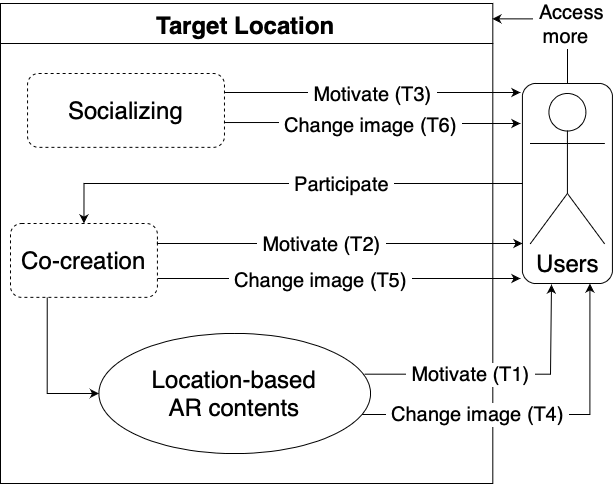
\includegraphics[width=0.8\columnwidth]{resources/5_experiment_and_results/proposed_framework_with_evaluation_targets.png}
    \caption{Proposed framework and targets to evaluate}
\end{figure}

\subsection{Evaluation of Motivation}

To evaluate targets about motivation, including T1, T2, T3 and T7, we adopted questions from Situational Motivation Scale (SIMS) \cite{guay_vallerand_blanchard_2000} for measurement.
SIMS contains four categories of motivation: 'Intrinsic motivation', 'Extrinsic motivation', and 'Amotivation', while in this study we specifically adopted 'Intrinsic motivation (IM)' and 'Amotivation (AM)'.
'Extrinsic motivation', including 'Identified regulation (IR)' and 'External regulation (ER)' are excluded since what we wanted to measure is the motivation induced by components in the proposed framework, instead of following any instruction, obligation, or any other external factors.
Questions we adopted from SIMS are listed in Appendix A.
Here we adopted 6 point scales to avoid ambiguous responses (where users keep choosing the middle item).

Cahyono et al. adopted SIMS with the use of Self-Determination Index (SDI) for scoring, which is calculated by the formula below:
\[ SDI = (2 * IM) + IR - ER - (2 * AM) \]
The higher the value of SDI, the more intrinsically motivated a person is \cite{cahyono_ludwig_2017}.
However, since we excluded IR and ER in this study, we conducted the scoring with:

\[ IM - AM \]

and composed a hypothesis for the scoring of motivation:

\begin{quote}
  Value of IM - AM measured with SIMS are positive for location-based AR, Co-creation, user-user interaction, and the combination of them.
\end{quote}

% \begin{quote}
%   \begin{itemize}
%     \item H1: For T1, the value of IM - AM measured with SIMS is positive.
%     \item H2: For T2, the value of IM - AM measured with SIMS is positive.
%     \item H3: For T3, the value of IM - AM measured with SIMS is positive.
%     \item H4: For T7, the value of IM - AM measured with SIMS is positive.
%   \end{itemize}
% \end{quote}

Besides the scales, we also prepared questions for free comments about motivation.

\subsection{Evaluation of Changes in Image}

To evaluate targets about changes in image of the campus, including T4, T5, T6 and T8,
we prepared a question with 5 point scale, described as follows:

\begin{quote}
  Does the image of the campus in your mind changed?
  \begin{enumerate}
    \item Not at all
    \item Only a little
    \item Somehow changed
    \item Changed a lot
    \item Completely changed
  \end{enumerate}
\end{quote}

Besides the scales, we also prepared questions for free comments about changes in image of the campus.

\subsection{Questionnaires}

Then we designed 4 questionnaires prepared for participants in an experiment conducted later (explanation in section 5.2). Each questionnaire corresponds to a factor listed as follows:

\begin{quote}
  Factors
  \begin{enumerate}
    \item Viewing location-based AR contents, the graffiti, in the campus
    \item Creating location-based AR contents, the graffiti, in the campus
    \item Interactions with other users
    \item Overall experience of using the prototype
  \end{enumerate}
\end{quote}

In each questionnaire, we asked questions about how the experience of the factor during the experiment affected one's motivation to access the campus, with questions introduced in Section 5.1.2, as well as changes in image of the campus in one's mind, with questions introduced in Section 5.1.3.
For example, Questionnaire 1 includes questions about the motivation and changes in image of the campus influenced by the experience of Factor 1: viewing location-based AR contents in the campus.

Results from Questionnaire 1 correspond to the evaluation of T1 and T4, Questionnaire 2 to T2 and T5, Questionnaire 3 to T3 and T6, and finally Questionnaire 4 to T7 and T8.
% In Questionnaire 1, 2 and 4, we also asked questions about participants' feeling of presence to check its relevance to the questionnaire's factor.
In Questionnaire 3, we also included questions about awareness of other users' existence and interaction with them, in order to confirm that the socializing mechanism functions effectively in the prototype.
Eventually, in each questionnaire, we also asked whether a participant, after attending the experiment, prefers our location-based AR prototype or a similar one without location-based features and AR effect but usable at home,
in order to make clear of the importance of location-based AR.

\section{Experiment}

At first, we conducted a preliminary survey with 3 participants trying the prototype in Waseda University Nishi-Waseda Campus for one week.
3 participants gave us positive responses about their motivation to access campus after experiencing the prototype.
We also improved the app based on their feedbacks, such as adding features that allow users to review/edit/delete their own graffiti.
The experiment lasted for 2 weeks. Participants include 14 males and 2 females, and all of them are in the age of 20s.
They are asked to use the prototype freely in the same campus at least twice a week.
Before the experiment, we asked participants about their frequencies of accessing the campus and the images of campus in their mind before and after the pandemic started spreading,
in order to understand how much impact the pandemic brought on each participant.
Instruction of using the prototype was also distributed before the experiment.
2 weeks later, after the experiment finished, participants were required to answer the questionnaires introduced in Section 5.1.

We also conducted a control experiment, with 3 males and 1 females participating in playing a similar prototype without location-based features and AR effect but usable at home for a week.
Then we asked them to fill in the same questionnaires.

\section{Results}
\subsection{Motivations}

Table 5.1 to 5.4 shows the evaluation results of motivation to access campus from Questionnaire 1 to 4 respectively.
All of them had positive values of either the average or the median of IM - AM, which verifies our hypothesis for the scoring of motivation.
In addition, among results from Table 5.1, 5.2 and 5.3, although they did not vary much, results by Factor 1 (mean of IM - AM: 1.6406, median of IM - AM: 1.6250) are the lowest,
and results by Factor 2 (mean of IM - AM: 1.9667, median of IM - AM: 2.0000) are the highest.
% This indicates that participation in Co-creation motivates the most, and viewing location-based AR contents motivates the least.
Notably, standard deviation of IM - AM by Factor 3 (value: 2.0743) is the highest and the only one higher than 2.0000.
% , indicating the variability in responses with regard to motivation influenced by interaction with other users.
Last but not least, in Table 5.4, results by Factor 4 (mean of IM - AM: 2.0156, median of IM - AM: 2.6250) had higher values than those by Factor 1 to 3, indicating that a combination of location-based AR contents, Co-creation and interaction has a better effect on improving motivation.

\begin{table}[h]
  \caption{Motivation to access campus influenced by Factor 1: viewing location-based AR contents}
    \label{table:1}
  \begin{tabular}{l || R{4cm} | R{3cm} | R{2.5cm}}
    \hline
    \rowcolor{lightgray}
          & \multicolumn{1}{c |}{Intrinsic motivation (IM)} & \multicolumn{1}{c |}{Amotivation (AM)} & \multicolumn{1}{c}{IM - AM}  \\
    \hline
    N      & 16     & 16     & 16      \\
    Mean   & 4.3906 & 2.7500 & 1.6406  \\
    Median & 4.3750 & 3.0000 & 1.6250  \\
    Min    & 3.0000 & 1.0000 & -1.5000 \\
    Max    & 6.0000 & 4.5000 & 5.0000  \\
    SD     & 0.7636 & 1.0124 & 1.5916  \\
    \hline
  \end{tabular}
\end{table}

\begin{table}[h]
  \caption{Motivation to access campus influenced by Factor 2: participation in Co-creation}
    \label{table:2}
  \begin{tabular}{l || R{4cm} | R{3cm} | R{2.5cm}}
    \hline
    \rowcolor{lightgray}
          & \multicolumn{1}{c |}{Intrinsic motivation (IM)} & \multicolumn{1}{c |}{Amotivation (AM)} & \multicolumn{1}{c}{IM - AM}  \\
    \hline
    N      & 15     & 15     & 15      \\
    Mean   & 4.4833 & 2.5167 & 1.9667  \\
    Median & 4.2500 & 2.5000 & 2.0000  \\
    Min    & 3.0000 & 1.0000 & -1.5000 \\
    Max    & 6.0000 & 4.5000 & 5.0000  \\
    SD     & 0.8044 & 1.0021 & 1.6767  \\
    \hline
  \end{tabular}
\end{table}

\begin{table}[h]
  \caption{Motivation to access campus influenced by Factor 3: interaction with other users}
    \label{table:3}
  \begin{tabular}{l || R{4cm} | R{3cm} | R{2.5cm}}
    \hline
    \rowcolor{lightgray}
          & \multicolumn{1}{c |}{Intrinsic motivation (IM)} & \multicolumn{1}{c |}{Amotivation (AM)} & \multicolumn{1}{c}{IM - AM}  \\
    \hline
    N      & 15     & 15     & 15      \\
    Mean   & 4.3833 & 2.5833 & 1.7200  \\
    Median & 4.7500 & 2.0000 & 1.8000  \\
    Min    & 2.0000 & 1.0000 & -2.0000 \\
    Max    & 6.0000 & 5.0000 & 5.0000  \\
    SD     & 1.1135 & 1.1286 & 2.0743  \\
    \hline
  \end{tabular}
\end{table}
  
\begin{table}[h]
    \caption{Motivation to access campus influenced by Factor 4: overall experience of the prototype}
      \label{table:4}
    \begin{tabular}{l || R{4cm} | R{3cm} | R{2.5cm}}
    \hline
    \rowcolor{lightgray}
          & \multicolumn{1}{c |}{Intrinsic motivation (IM)} & \multicolumn{1}{c |}{Amotivation (AM)} & \multicolumn{1}{c}{IM - AM}  \\
    \hline
    N      & 16     & 16     & 16      \\
    Mean   & 4.5469 & 2.5313 & 2.0156  \\
    Median & 4.6250 & 2.2500 & 2.6250  \\
    Min    & 3.0000 & 1.0000 & -2.0000 \\
    Max    & 6.0000 & 5.0000 & 5.0000  \\
    SD     & 0.8328 & 1.0950 & 1.8108  \\
    \hline
  \end{tabular}
\end{table}

We also collected free comments about motivation in each questionnaire. In Questionnaire 1 we received responses for IM, including 'I become curious about other people's graffities and their comments on my drawings',
'I feel more creative and fun by sharing works with others', 'It is fun to secretly see my friends' drawings', 'Sometimes I felt connected to other students',
which we considered are related to interaction with users as well.
In Questionnaire 3 we received responses with obviously opposite attitudes: one states 'I feel like I can make friends with this' for IM and another one answered 'Interaction with user can be done online too in my opinion' for AM.
% This corresponds to the variability with regard to motivation influenced by interaction with other users, which we observed from the evaluation results of Table 5.3 and mentioned in the last paragraph.
Questionnaire 4 collected a response for AM that states '... as long as the social distance (due to the pandemic) exists, there may be many constraints on AR since it mainly bases on reality',
pointing out the limitation of AR under pandemic circumstances.

\subsection{Image of the campus}

Table 5.5 shows the evaluation results of changes in image of the campus from Questionnaire 1 to 4.
Each factor resulted in a mean value between 2 (Changed a little) and 3 (Somehow changed) as well as a median value equal to 3 (Somehow changed).
Among Factor 1, 2 and 3, Factor 3 resulted in the highest mean value (2.8667), and Factor 1 resulted in the lowest one (2.6875),
% indicating that interaction among users changed the image the most, and viewing location-based AR contents changed the least.
while Factor 3 had the highest standard deviation (0.8338), indicating the disagreement of attitudes among participants toward user-user interaction.
In addition, results by Factor 4 had higher values than those by Factor 1 to 3, indicating that a combination of three of the components again has a better effect on changing the image.

We also collected free responses, listed in Appendix B. Most of the responses express positive changes, such as "I used to feel that the campus was quiet and there was little interaction between people, but through this content, I learned that I could interact with strangers, and my image of the campus became more sociable.",
"I hadn't had a chance to take a good look at the campus, so it was refreshing.", "I started to think sometimes about what things on campus could look like.", "I developed a common feeling that we were all students at the same university.",
while there are also negative opinions, such as "The campus became a little more fun, but it wouldn't have changed my overall image.", "To me, it was just an application on phone where I can draw and see others' works", "I thought that since the interaction was with people, it had little impact on the image of the campus.".
There are positive responses describing a more sociable image of the campus or the feeling of connection with other students, while some negative responses doubted the relation between users and image of a place, which correspond to the high but variant results of Factor 3: interaction among users.

\begin{table}[h]
  \caption{Changes in image of the campus by different factors, scaled from 1 (Not at all) to 5 (Completely changed)}
    \label{table:5}
  \begin{tabular}{l || R{3.5cm} | R{2.5cm} | R{2cm} | R{2cm}}
    \hline
    \rowcolor{lightgray}
          & \multicolumn{1}{C{3.5cm} |}{1. View location- \newline based AR contents} & \multicolumn{1}{C{2.5cm} |}{2. Participate \newline in Co-creation} & \multicolumn{1}{C{2cm} |}{3. User-user \newline interaction} & \multicolumn{1}{C{2cm}}{4. Overall \newline experience} \\
    \hline
    N      & 16     & 15     & 15     & 16     \\
    Mean   & 2.6875 & 2.7333 & 2.8667 & 2.8750 \\
    Median & 3.0000 & 3.0000 & 3.0000 & 3.0000 \\
    Min    & 2.0000 & 2.0000 & 2.0000 & 2.0000 \\
    Max    & 4.0000 & 4.0000 & 4.0000 & 4.0000 \\
    SD     & 0.6021 & 0.5936 & 0.8338 & 0.8062 \\
    \hline
  \end{tabular}
\end{table}

\subsection{User-user Interaction}

In Questionnaire 3, we also evaluated participants' sense of other users' existence and interaction,
and the results are displayed in Table 5.6. Among 1 (Disagree) to 6 (Agree), mean and median values of both existence and interaction are more than or equal 4.
% indicating that the protoype succeeded to make users feel others' existence and build interaction between them.
The free responses we collected contain "I went to use this system with another participant. We were playing a game of guessing which graffiti each other had drawn" and "I used it with my classmates, and we talked about what we were drawing".
% which described real cases of interaction among users with our framework.

\begin{table}[h]
  \caption{Sense of other users' existence and interaction, scaled from 1 (Disagree) to 6 (Agree)}
    \label{table:6}
  \begin{tabular}{l || R{5cm} | R{5.5cm}}
    \hline
    \rowcolor{lightgray}
          & \multicolumn{1}{C{5cm} |}{I felt existence \newline of other users} & \multicolumn{1}{C{5.5cm}}{It felt like I am \newline interacting with other users} \\
    \hline
    N      & 15     & 15     \\
    Mean   & 4.5333 & 4.0000 \\
    Median & 5.0000 & 4.0000 \\
    Min    & 3.0000 & 2.0000 \\
    Max    & 6.0000 & 6.0000 \\
    SD     & 0.9155 & 1.3093 \\
    \hline
  \end{tabular}
\end{table}

% \subsection{Revelance of Feeling of Presence}

\subsection{Comparison with situation without location-based AR}

Table 5.7 shows the evaluation results of participants' preference between prototype at campus or situation at home by different factors.
For each factor, the mean value is between 4 and 5, and the median value equals 5 or 6. This indicates a higher preference for our prototype where location-based AR features is implemented.
We also collected free responses about the preference, with some of which listed in Appendix C.
Responses that prefer the case at campus mainly express that the prototype at campus with location-based AR creates more fun, enables exploration of different perspectives and sense of realism, or provides chances to meet other users in reality.
Responses that prefer the case at home mainly point out difficulties to use at campus due to the environment or people passed by, question the necessary of interacting with other users in reality, or express the weariness of physically traveling around the campus.

\begin{table}[h]
  \caption{Preference between prototype at campus or situation at home by different factors, scaled from 1 (At home) from 7 (At campus)}
    \label{table:7}
  \begin{tabular}{l || R{3.5cm} | R{2.6cm} | R{2cm} | R{2cm}}
    \hline
    \rowcolor{lightgray}
          & \multicolumn{1}{C{3.5cm} |}{Viewing location- \newline based AR contents} & \multicolumn{1}{C{2.6cm} |}{Participation \newline in Co-creation} & \multicolumn{1}{C{2cm} |}{User-user \newline interaction} & \multicolumn{1}{C{2cm}}{Overall \newline experience} \\
    \hline
    N      & 16     & 15     & 15     & 16     \\
    Mean   & 4.8125 & 4.8667 & 4.6000 & 4.7500 \\
    Median & 5.0000 & 6.0000 & 5.0000 & 6.0000 \\
    Min    & 1.0000 & 1.0000 & 1.0000 & 1.0000 \\
    Max    & 7.0000 & 7.0000 & 7.0000 & 7.0000 \\
    SD     & 1.6419 & 1.8074 & 1.6388 & 1.8074 \\
    \hline
  \end{tabular}
\end{table}

In the control experiment where participants used another prototype without location-based AR features, evaluation of motivation shows negative evaluation values,
and evaluation results of image changing of campus are less significant than the results from the formal experiment.
Results of motivation and image changing are listed in Table 5.8 and 5.9 respectively.
Since there were only several participants, we did not conduct statistical analysis in this control experiment; the results are only for reference.

% table: mean of each IM & AM & IM-AM, mean of each image changing
\begin{table}[h]
  \caption{Motivation to access campus influenced by different factors in control experiment (only mean values)}
    \label{table:8}
  \begin{tabular}{l || R{3.4cm} | R{2.6cm} | R{2cm} | R{1.9cm}}
    \hline
    \rowcolor{lightgray}
          & \multicolumn{1}{C{3.4cm} |}{View location- \newline based AR contents} & \multicolumn{1}{C{2.6cm} |}{Participate \newline in Co-creation} & \multicolumn{1}{C{2cm} |}{User-user \newline interaction} & \multicolumn{1}{C{1.9cm}}{Overall \newline experience} \\
    \hline
    N       & 4      & 3       & 3       & 3       \\
    IM      & 3.6875 & 2.4167  & 2.7500  & 3.1667  \\
    AM      & 3.5000 & 4.4167  & 3.1667  & 3.9167  \\
    IM - AM & 0.1875 & -2.0000 & -0.4167 & -0.7500 \\
    \hline
  \end{tabular}
\end{table}

\begin{table}[h]
  \caption{Changes in image of the campus by different factors in control experiment, scaled from 1 (Not at all) to 5 (Completely changed)}
    \label{table:9}
  \begin{tabular}{l || R{3.5cm} | R{3cm} | R{2cm} | R{2cm}}
    \hline
    \rowcolor{lightgray}
          & \multicolumn{1}{C{3.5cm} |}{View location- \newline based AR contents} & \multicolumn{1}{C{3cm} |}{Participate \newline in Co-creation} & \multicolumn{1}{C{2cm} |}{User-user \newline interaction} & \multicolumn{1}{C{2cm}}{Overall \newline experience} \\
    \hline
    N      & 4    & 3    & 3    & 3    \\
    Mean   & 2.25 & 3.00 & 2.00 & 2.00 \\
    \hline
  \end{tabular}
\end{table}

About preference, we received free responses including "Doing this at home is more like drawing something on my picture. I don't feel fun drawing on it.", "I think that's the reason why AR is needed...? To explore somewhere that you can't actually visit", 
"AR seems to more interesting. There are many other interesting things to do at home." and "I personally prefer directly interacting with the users (person to person)", 
which show more interests in a situation with location-based AR than their non-AR experience in the control experiment.
